\documentclass{paper}

\usepackage{graphicx}
\usepackage{tabularx}

\title{Measurement of Energy Loss in the ADS FFAG Foil}
\author{Chris Rogers }

\begin{document}

\maketitle

\section{Data Taking}
The principle of the experiment is to measure the synchronous phase of the beam
as a function of RF voltage. When energy is "just" returned to the beam, the
sychronous phase should be 90$^{o}$.

A first dataset was taken on the afternoon of Friday 4th April, 2014. During 
that data taking the ion source was not performing well. Subsequent to the data 
taking the foil was found to have torn.

A second dataset was taken on the afternoon of Tuesday 24th June, 2014. The
orbital frequency was measured as 1.577 MHz and this was used as the RF 
frequency. The beam could not be injected over 6.6 $\mu$s as this caused 
saturation in the beam loss monitors so a shorter injection period was used 
\emph{(what period?)}.

Due to the problems with the first dataset, that data is not studied in this
analysis. Instead only the data taking during the June running is considered.

\section{Input Signals}
The analysis followed several stages. The time of the peaks in the RF signal and 
the bunch monitor signal S12 was calculated. The peak to peak time difference
was studied in each signal to understand the stability of the signal and then 
used to calculate RF frequency. The time difference between adjacent peaks of 
the two signals was then studied to identify beam capture behaviour. The peak to
peak voltage difference on the RF signal was used to calculate the RF voltage. 
The RF voltage was compared with the difference between time of RF signal and
beam signal, and the resulting relationship was used to infer an energy loss.

$10^6$ counts were read out, with time between counts of 0.2 ns. The data 
was recorded by averaging over 128 ion source pulses.

\subsection{Beam Monitor DC Signal}
The beam monitor measures the wall current induced by the passage of the beam.
The beam monitor acts as a capacitor; the wall current leads to a build up of
charge on the beam monitor, creating an induced voltage. By measuring this 
induced voltage we get a measurement like 

\begin{equation}
\int I/RC dt
\end{equation}

\emph{what is the time constant?}

\subsection{Beam Monitor AC Signal}
The "DC" signal is passed through a high-pass filter so that only the high-
frequency part of the "DC" signal i.e. the changes in the DC signal are read 
out. This is called the beam monitor "AC" signal. \emph{rogers guess}

\subsection{RF Signal}
The RF signal was generated by means of a pick-up in the RF cavity.

\subsection{Example signals}

\begin{figure}
		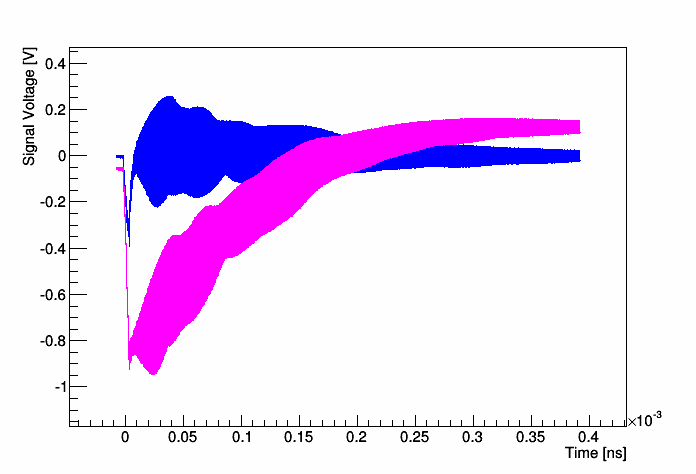
\includegraphics[width=0.5\textwidth]{images/v=7_18_signal_full}
		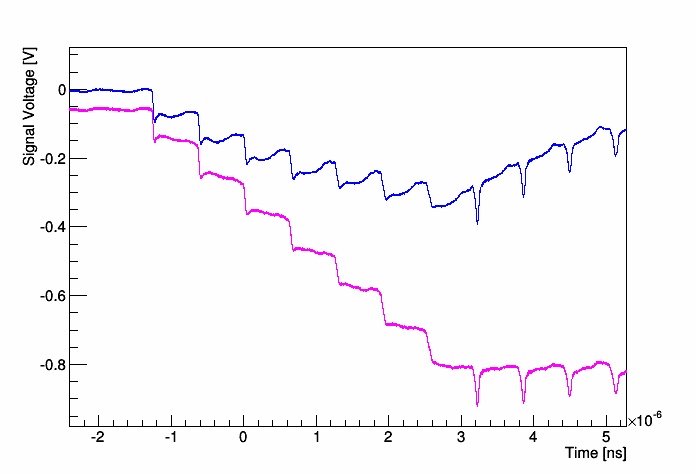
\includegraphics[width=0.5\textwidth]{images/v=7_18_signal_injection}
		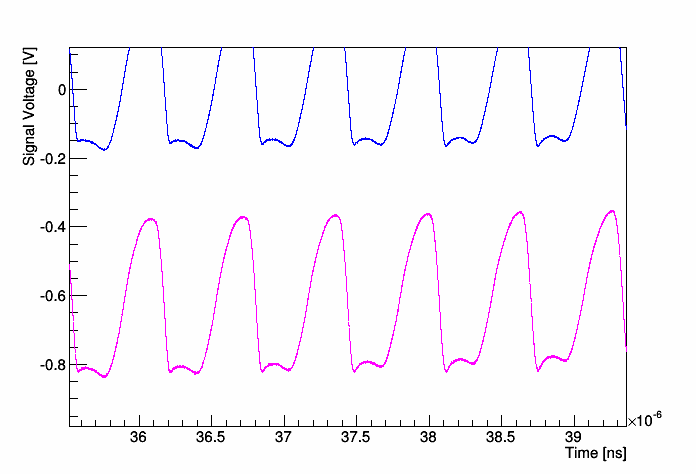
\includegraphics[width=0.5\textwidth]{images/v=7_18_signal_middle}
		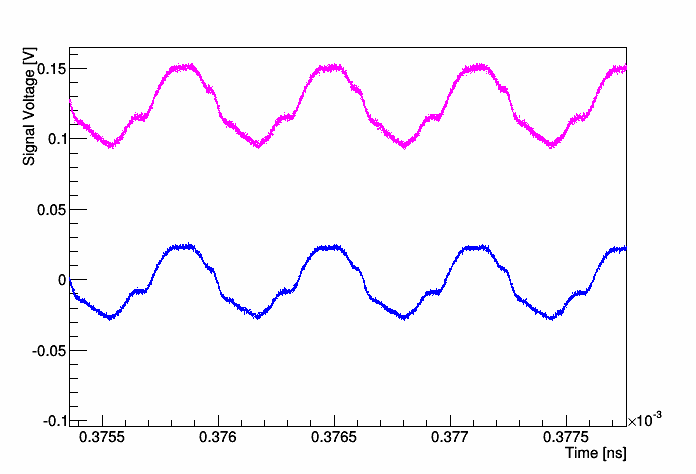
\includegraphics[width=0.5\textwidth]{images/v=7_18_signal_end}
	\caption{Example of measured DC (pink) and AC (blue) signals. From top to 
           bottom: full signal; signals around injection; signals in the middle
           of the cycle; signals at the end of the cycle. Note a negative signal
           corresponds to a positive current.}
	\label{fig:bm_signals}
\end{figure}

A sample set of signals is shown in Fig. \ref{fig:bm_signals}. Near to injection the
DC component of the signal is observed to be reduced in the AC signal. 

A false peak is observed around injection in the AC signal, and it is thought that this 
is an artefact of the filtering electronics. \emph{really?}

In the middle of the cycle the double peak is noted. This will be discussed 
later. At the end of the cycle, signal noise becomes significant.

\begin{figure}
		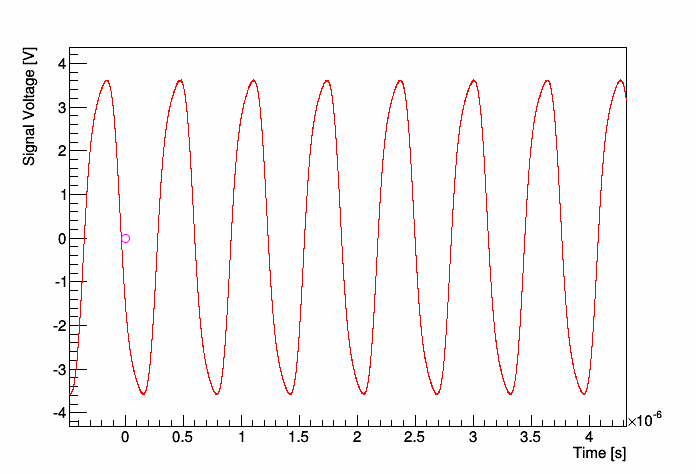
\includegraphics[width=0.5\textwidth]{images/v=7_18_signal_rf}
	\caption{Example of measured RF signal.}
	\label{fig:rf_signal}
\end{figure}

A sample RF signal is shown in Fig. \ref{fig:rf_signal}. It is noted that the
RF signal is not a precise sinusoid. \emph{Is this a feature of the electronics?
Is the cavity Q low enough for that?}

\section{Measurement of Bunch Phase}

The algorithm used to find the bunch phase relative to the RF cavity is next
described.

\subsection{Peak Finding Algorithm}
Peaks were found in the first instance by smoothing the data using a Gaussian
function with standard deviation 50 ns. This was followed by a search for peaks 
performed by looking for the peak values within a 50 ns window. The window was
advanced in steps of 25 ns and the peak value was recorded within the window. 
Peak values at the window edge were ignored. Where multiple peaks were found
with this algorithm, they were recorded.

This initial estimate was refined by fitting a quadratic function to the
raw (unsmoothed) data points in the region of the peak. The points used for 
fitting were dynamically selected by requiring that the residuals of the fit
$x(fit)-x(data)$ within some window should not have a standard deviation much 
larger than the estimated standard deviation of the data very close to the peak. 
The window was made smaller until this condition was met. The time and magnitude
of the peak, $t_p, y_p$ were estimated from the fit parameters, according to
\begin{eqnarray}
y &=& a_0 + a_1 t + a_2 t^2 \\
t_p &=& -\frac{a_1}{2a_2}  \\
y_p &=& -\frac{a_1^2}{4a_2}+a_0
\end{eqnarray}
The errors were calculated using the standard relationship
\begin{eqnarray}
\mathbf{V}(t_p, y_p) = \mathbf{J} \mathbf{V}(\vec{a}) \mathbf{J^T}
\end{eqnarray}
where $\mathbf{V}$ are the covariance matrices. $\mathbf{V}(\vec{a})$ was 
calculated by taking the numerical derivative of the fit parameters with respect 
to the $\chi^2$, which is done  automatically by the ROOT software used for 
fitting. $\mathbf{J}$ is the Jacobian for $(t_p(\vec{a}), y_p(\vec{a}))$, given
by
\begin{equation}
\mathbf{J} = \left(\begin{array}{ccc}
    0 & -1/2a_2 & a_1/2a_2^2 \\
    1 & -a_1/2a_2 & a_1^2/4a_2^2
\end{array}\right)
\end{equation}

\subsection{RF Signal Peaks}
The magnitude and time of peaks and troughs was calculated using the peak 
finding algorithm outlined above. The time difference between adjacent peaks is
shown in Fig. \ref{fig:rf_peak_deltas}, both as a function of time and in
projection. The 0.2 ns divisions are a consequence of the peak finding 
algorithm. The peak finding algorithm can be made more accurate 
(but it probably doesn't really matter).

\begin{figure}
		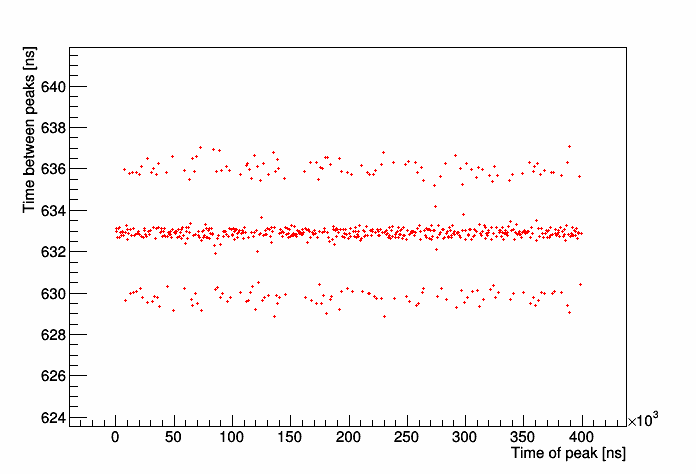
\includegraphics[width=0.5\textwidth]{images/v=7_18_rf_peak_deltas}
		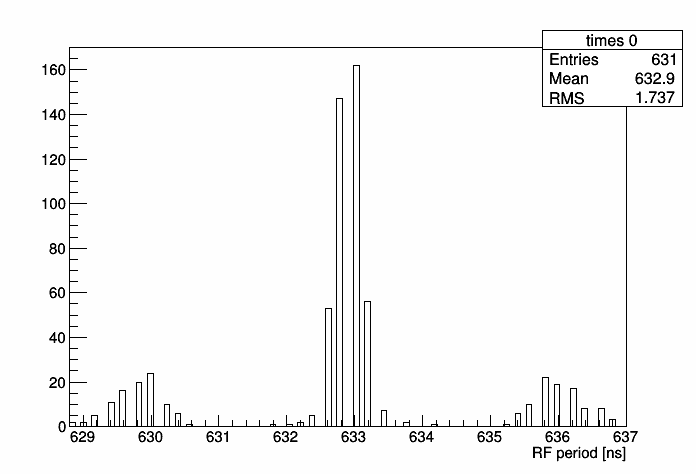
\includegraphics[width=0.5\textwidth]{images/v=7_18_rf_period_distribution}
	\caption{Distribution of time between adjacent RF peaks (top) as a function of
          time (bottom) projection of top histogram. The 0.2 ns arises from the
          peak finding algorithm. Side bands are visible 3 ns from the main
          peak; the source is not known.}
	\label{fig:rf_peak_deltas}
\end{figure}

The frequency is seen to be stable across many pulses, to within the
measurement error. There appear to be side-bands a few ns away from the main
peak and this is also observed for other samples. To give an order of magnitude 
for the significance of these features, it is noted that simulation through the 
field map with $F = 810 A$ and $D = 1020 A$
\begin{equation}
dT/dE = 23.07 ns/MeV
\end{equation}
\emph{Could check for this feature with FFT - just in case it is the fitting
algorithm doing it.}

The mean RF period is measured as 632.9 +/- 0.1 ns. The RF frequency is 
consistent at different voltages.

The RF voltage is taken as half the peak to trough distance. The RF voltage as a
function of time within the sample is shown in Fig. \ref{rf_peak_magnitudes}. 
The dogleg feature is noted. The absolute magnitude of the "dogleg" varies 
between 0.002 and 0.008 V, the fractional magnitude staying less tan around 1 
$\%$. The width of the peak spread is consistent with errors reported by the
peak fitting algorithm.

\begin{figure}
		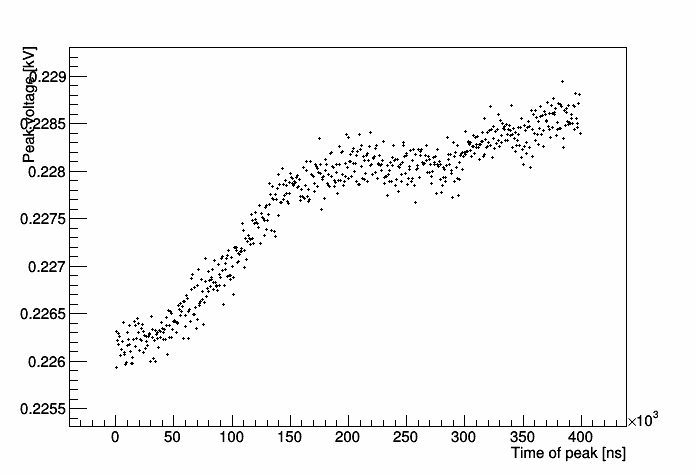
\includegraphics[width=0.5\textwidth]{images/v=0_46_rf_magnitude}
		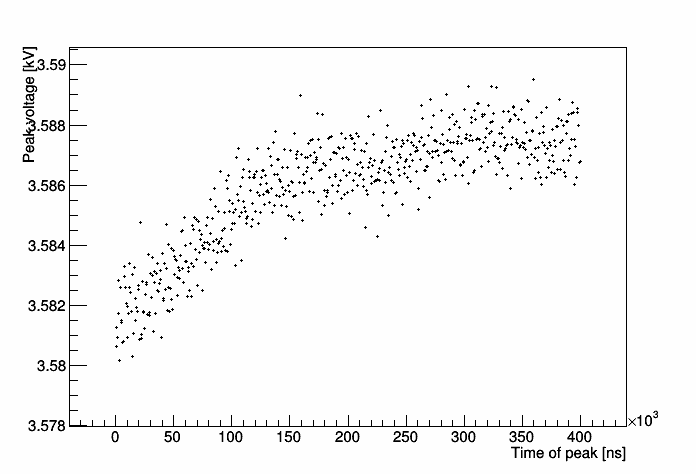
\includegraphics[width=0.5\textwidth]{images/v=7_18_rf_magnitude}
	\caption{Peak voltage (top) for 0.229 V and (bottom) for 3.589 V signals. The 
           dogleg feature is noted, where the RF voltage takes some time to come
           up to a flat top.}
	\label{fig:rf_peak_magnitudes}
\end{figure}


The average RF voltages (half peak to trough for each sample) are listed below:
\begin{itemize}
\item 0.101
\item 0.16
\item 0.229
\item 0.308
\item 0.406
\item 0.523
\item 0.664
\item 0.835
\item 1.023
\item 1.241
\item 1.504
\item 1.792
\item 2.106
\item 2.318
\item 2.545
\item 2.692
\item 2.876
\item 3.057
\item 3.232
\item 3.407
\item 3.589
\end{itemize}

\subsection{Bunch Monitor Signal}
For higher RF voltages, the beam is well captured and the peak-to-peak period is
roughly constant across a reasonable range. For lower voltages the beam is less 
well captured and the peak-to-peak period shows much greater variation. Even for 
the case where the beam is well captured, the spread in peak-to-peak times is 
larger than the calculated error in the peak finder, indicating that there may 
be some debunching or other behaviour occurring.

Bunch monitor signals for a selection of the measured data sets are shown in 
Fig. \ref{fig:bm_signal_periodic_captured} and Fig. 
\ref{fig:bm_signal_periodic_not_captured}. Further interpretation of the
bunch monitor signals is given by comparison to Monte Carlo in section 
\ref{sec:mc}

\begin{figure}
		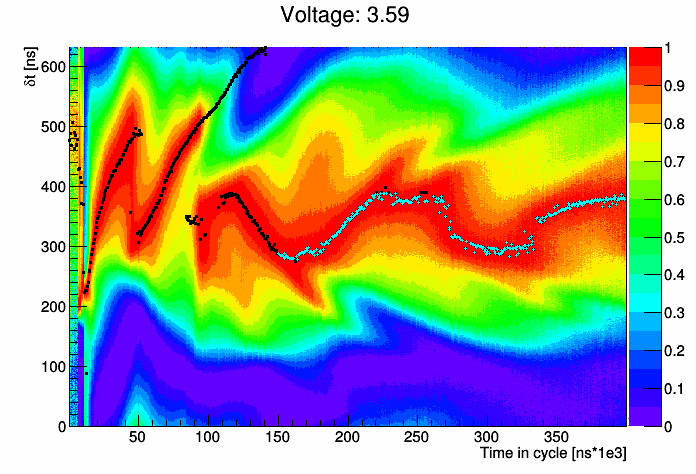
\includegraphics[width=0.5\textwidth]{images/V=7_18_fitted_bpm_to_rf_deltas}
		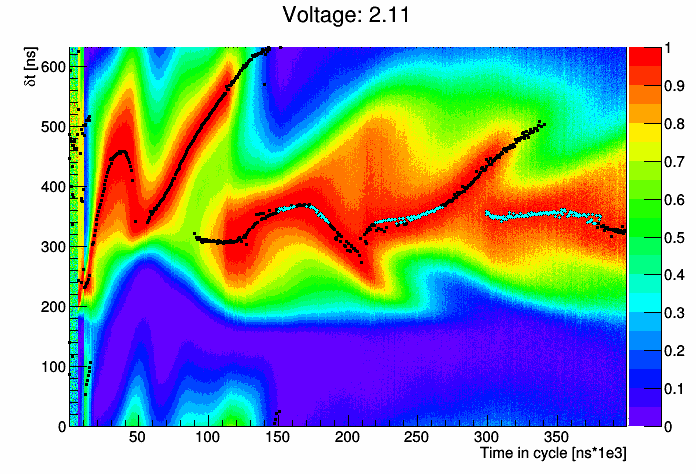
\includegraphics[width=0.5\textwidth]{images/V=4_21_fitted_bpm_to_rf_deltas}
		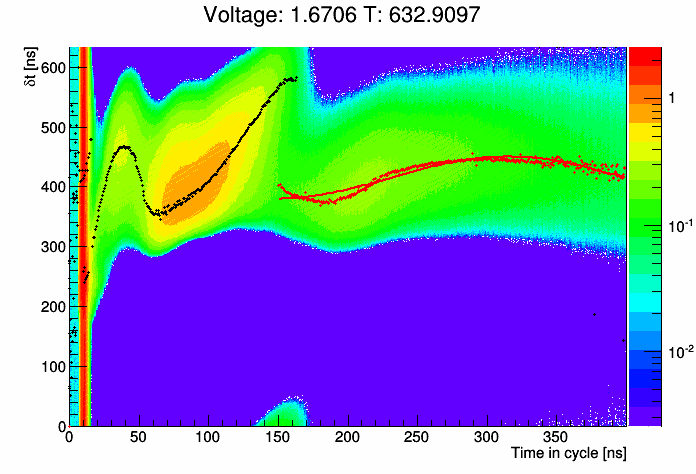
\includegraphics[width=0.5\textwidth]{images/V=1_67_fitted_bpm_to_rf_deltas}
	\caption{BPM signal for RF voltages where the beam is considered to be
           captured. The colours show AC signal voltage. $\delta t$ is the time
           relative to the most recent RF peak. The points show the position of
           the measured peaks in the beam current. Red points are those which
           are included in the analysis. Early in the cycle the beam is assumed
           to be not captured. The red line corresponds to a sine curve fit to
           the red points. The units for the abscissa are $1e3 ns$.}
	\label{fig:bm_signal_periodic_captured}
\end{figure}

\begin{figure}
		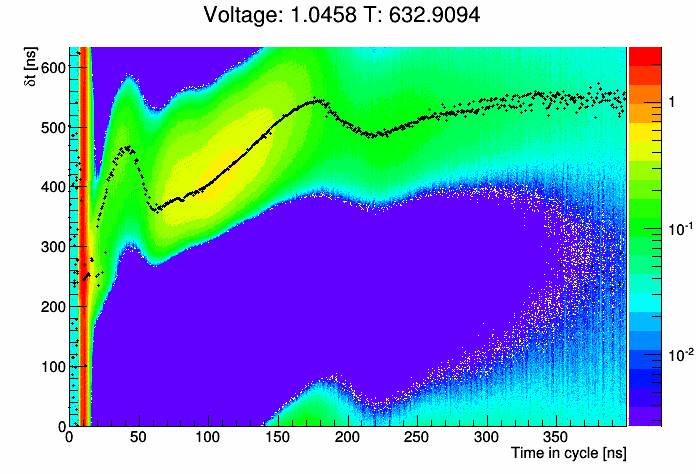
\includegraphics[width=0.5\textwidth]{images/V=1_05_fitted_bpm_to_rf_deltas}
		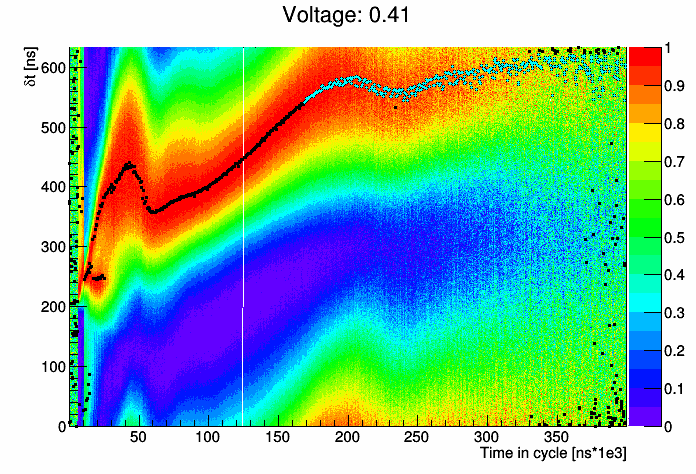
\includegraphics[width=0.5\textwidth]{images/V=0_81_fitted_bpm_to_rf_deltas}
		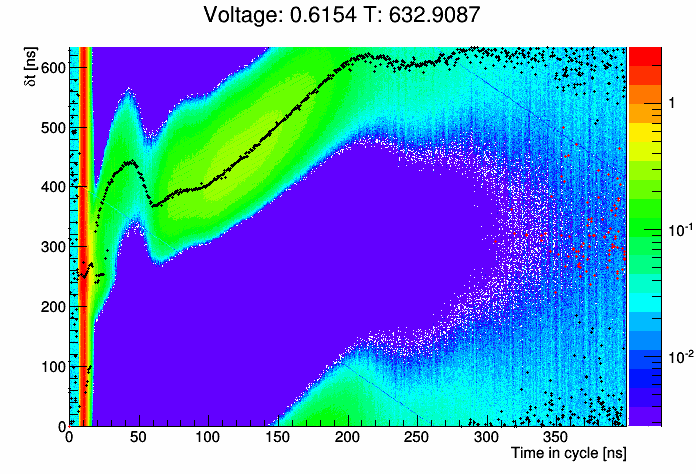
\includegraphics[width=0.5\textwidth]{images/V=0_62_fitted_bpm_to_rf_deltas}
	\caption{BPM signal for RF voltages where the beam is not considered to be
           captured. The colours show AC signal voltage. $\delta t$ is the time
           relative to the most recent RF peak. The points show the position of
           the measured peaks in the beam current. The units for the abscissa
           are $1e3 ns$.}
	\label{fig:bm_signal_periodic_not_captured}
\end{figure}

\subsection{RF Phase of Captured Bunch}
The phase of the measured peaks in the bunch monitor signal are used to 
calculate the RF phase of the captured bunch. The bunch is considered to be
captured when the  bunch peak falls  with in a window defined by 
$1.5e5 < t [ns] < 4.0e5$ and $200 < \delta t [ns] < 500 $.

The bunch phase is calculated using one of two algorithms.
\begin{itemize}
\item Sinusoidal fit: A sinusoidal fit, as shown in Fig. 
\ref{fig:bm_signal_periodic_captured}, is made to the peaks of the captured
bunch. The error is taken to be the error on the fit (\emph{wrong, should be
based on chi2 I think.}).
\item Mean fit: The average $\delta t$ of the captured bunch peaks  is 
calculated. The error is taken to be RMS $\delta t$.
\end{itemize}
The phase is calculated from $\delta t$ by the relation
\begin{equation}
\phi = 2 \pi \delta t / \tau
\end{equation}
where $\tau$ is the RF period. The resultant relationship between bunch phase 
and voltage is shown for the two different algorithms in 
\ref{fig:rf_phase_to_voltage}.

In order to calculate a measured thickness of the foil, the RF phase is compared
to the peak voltage. When the beam is coasting, the energy returned to the beam
should balance the energy lost on the foil. Hence

\begin{equation}
V_0 = c\delta W \sin (\phi_s+d\phi).
\end{equation}

where $V_0$ is the peak voltage, $c$ is a calibration constant that scales the
pickup voltage to the voltage experienced by a proton in the FFAG, $\delta W$ is
the energy lost on the foil, $\phi_s$ is the reference phase and $d\phi$ is a 
calibration constant representing azimuthal offset of the RF cavity and the 
bunch monitor, cable lengths and any associated electronics signal delays.

The calibration constant $c$ has value 1e3 (with what errors?)

The calculated fit parameters for the two cases are listed below.
\begin{itemize}
\item Sinusoidal fit: $dW = -1.2105 +/- 0.0021$ keV, $d\phi = 0.233 +/- 0.000955$ rad
\item Mean fit: $dW =-0.85079 +/- 0.0017$ keV, $d\phi = 0.0752 +/- 0.000616$ rad
\end{itemize}

\begin{figure}
		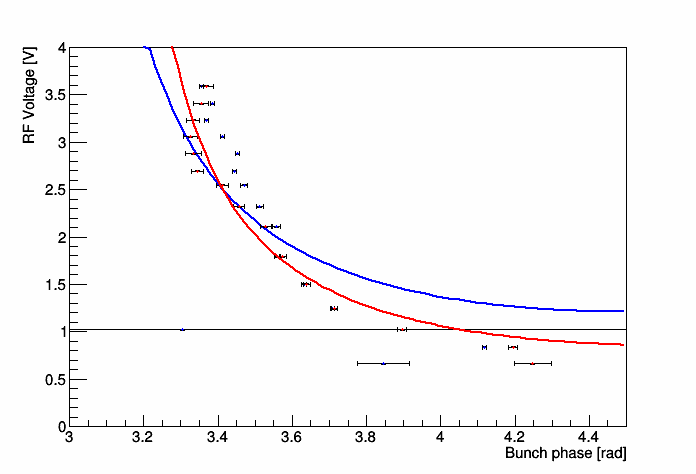
\includegraphics[width=1.0\textwidth]{images/synchronous_phase_vs_voltage}
	\caption{Measured synchronous phase relative compared to RF peak voltage for
   (red) mean fit method (blue) sinusoidal fit method. See text for details on
   the different methods and corresponding fit parameters.}
	\label{fig:rf_phase_to_voltage}
\end{figure}

\subsection{Measured Thickness}
We compare the measured energy lost in the foil with the Bethe-Bloch model 
\cite{PDG} and the GEANT4 QGSP energy loss model \cite{GEANT4} to deduce a 
measured foil thickness. The design thickness is 20 [$\mu g/cm^2$].

\begin{table}
\begin{center}
\begin{tabular}[\linewidth]{l|cc}
               & Bethe Bloch       & Geant4 QGSP \\
\hline
Mean energy loss &                 &
\hline
Sinusoidal fit & 35.6 $\mu g/cm^2$ & 38.4 $\mu g/cm^2$ \\
Mean fit       & 27.0 $\mu g/cm^2$ & 25.0 $\mu g/cm^2$ \\
\end{tabular}
\caption{Measured thickness of the foil.}
\end{center}
\end{table}

\section{Comparison to Monte Carlo}
\label{sec:mc}
A beam was simulated in the FFAG. Particles were thrown with initial 
time distributed randomly over a given time interval (0, 6400) ns and with no 
energy spread. The particle positions, momenta and times were subsequently 
recorded each time they were simulated crossing an output plane (i.e. once per 
turn). Unless specified stochastic processes are disabled - the particles only
experience mean energy loss and no scattering.

A sample simulated data set is shown in Fig. \ref{fig:nominal_mc}. The beam has
initially no energy spread and fills the RF period completely (100 $\%$ phase
spread). In time, the bunch can be seen to be compressed by the RF focussing with
a focussing period of about 100 $\mu s$. Some filamentation is observed of the
beam that is not caught in the RF bucket.

\begin{figure}
		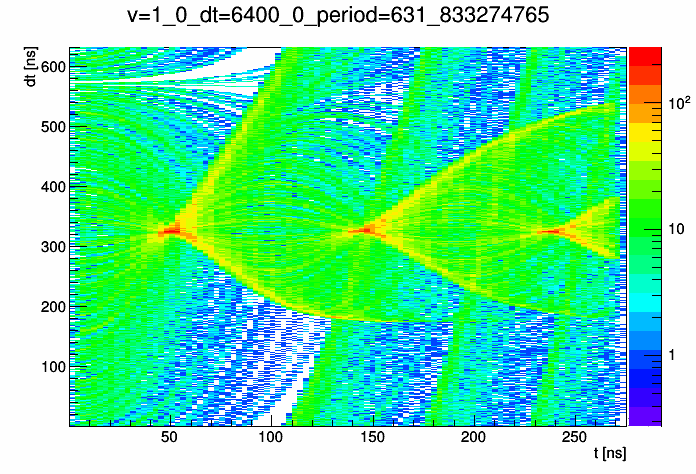
\includegraphics[width=0.5\textwidth]{images/time_vs_dt_v=1_0_dt=6400_0_period=631_833274765}
		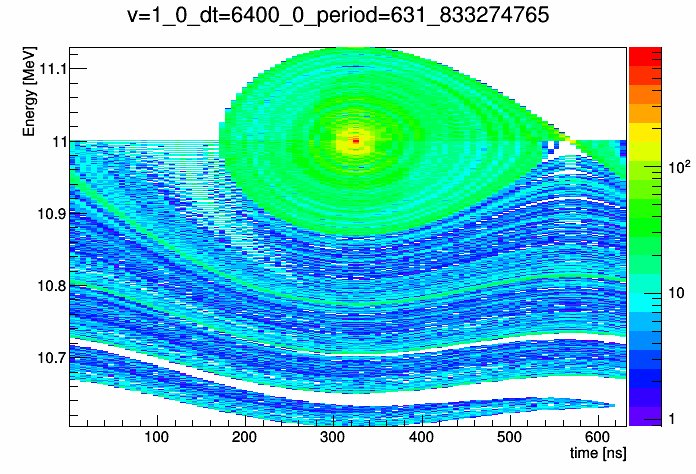
\includegraphics[width=0.5\textwidth]{images/time_vs_energy_v=1_0_dt=6400_0_period=631_833274765}
	\caption{Monte Carlo simulation of a nominal bunch. (Left) number of particles
           passing through the output plane in a given time bin (Right) Total 
           time vs energy for a nominal bunch. The units for the abscissa are
           $1e3 ns$.}
	\label{fig:nominal_mc}
\end{figure}

\subsection{Sensitivity to RF Voltage}


\subsection{Sensitivity to Injection Interval}

\begin{figure}
		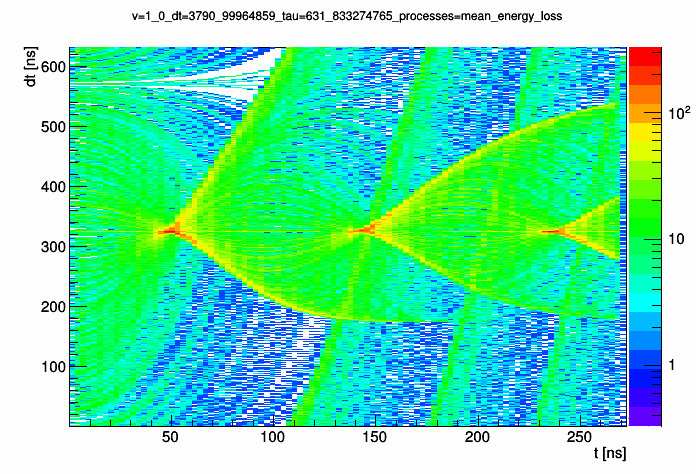
\includegraphics[width=0.5\textwidth]{images/time_vs_dt_v=1_0_dt=3790_99964859_tau=631_833274765_processes=mean_energy_loss}
		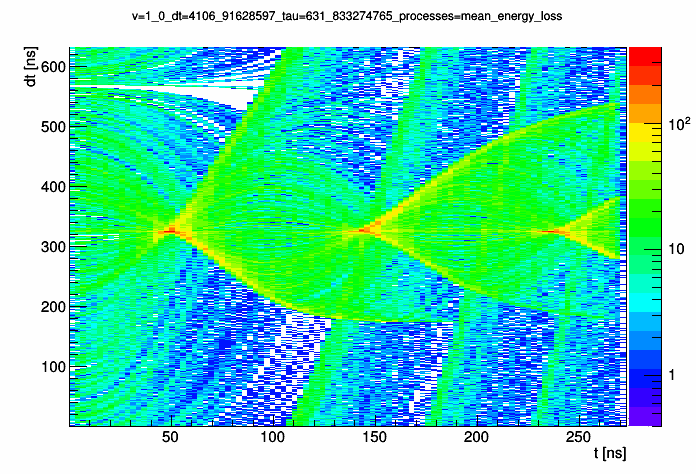
\includegraphics[width=0.5\textwidth]{images/time_vs_dt_v=1_0_dt=4106_91628597_tau=631_833274765_processes=mean_energy_loss}
	\caption{Simulation with variable injection interval (left) injection interval
           6 turns (right) injection interval 6.5 turns. The units for the
           abscissa are $1e3 ns$.}
	\label{fig:mc_injection_interval}
\end{figure}

During this study, the beam was injected over several turns. If the beam 
injection is not an integer number of turns, there will be a fractional surplus
during part of the turn. One may speculate that this causes a bunch-like feature
in the longitudinal distribution.

The ring was simulated with an injection interval of 6 turns and 6.5 turns, as
shown in Fig. \ref{fig:mc_injection_interval}. No effects are visible on the 
beam due to the variable injection interval.

\subsection{Sensitivity to Stochastic Processes}

\begin{figure}
		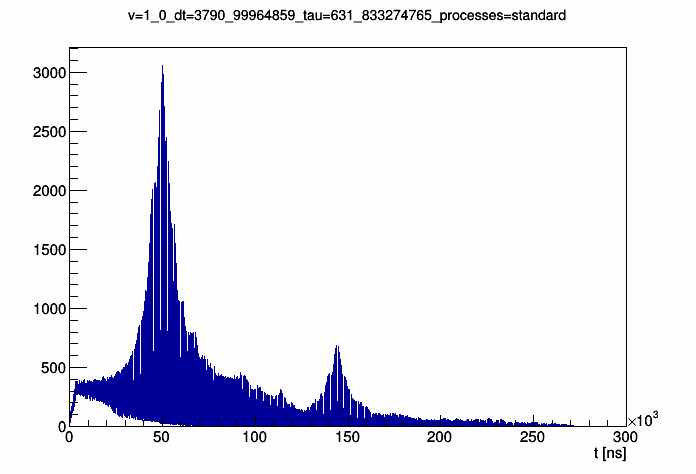
\includegraphics[width=0.5\textwidth]{images/beam_monitor_v=1_0_dt=3790_99964859_tau=631_833274765_processes=standard}
		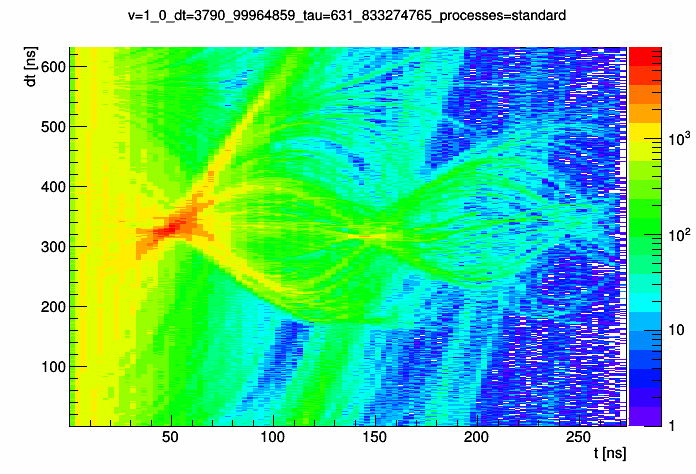
\includegraphics[width=0.5\textwidth]{images/time_vs_dt_v=1_0_dt=3790_99964859_tau=631_833274765_processes=standard}
	\caption{Simulation with all GEANT4 QGSP physics processes enabled: (left)
           number of muons crossing an output plane in a time step, as a 
           function of time; (right) number of muons crossing an output plane in
           a time step, as a function of time and phase. The 
           units for the abscissa are $1e3 ns$.}
	\label{fig:mc_stochastic processes}
\end{figure}

The effect of stochastic processes on the beam can be seen in Fig. 
\ref{fig:mc_stochastic processes}. The behaviour of the beam longitudinally
looks similar; there is now significant beam loss during the cycle,
which is thought to be caused by protons scattering vertically until the foil 
holder is hit.

\subsection{Sensitivity to RF Frequency}


\subsection{Sensitivity to Energy Spread}


\section{Discussion}

\end{document}

